\documentclass[main.tex]{subfiles}
\begin{document}

\chapter{Source foils design optimisation}


%\begin{flushright}
%\textit{The only thing that could save them was selenium.}\\
%Isaac Asimov, \textit{I, Robot, Runaround}.
%\end{flushright} 


\NI Sensitivity studies of the SuperNEMO experiment have shown that to reach a sensitivity of $\sim$ 10$^{\text{26}}$~y in 500~kg~$\times$~y of exposure with $^{\text{82}}$Se, the radio-purity level of the source foil in $^{\text{208}}$Tl and $^{\text{214}}$Bi must be better than respectively 2~$\mu$Bq/kg and 10~$\mu$Bq/kg [ref]. In order to measure these very low contaminations, the collaboration build the BiPo detector as explained in Section~\ref{sec:SourceFoilsSN}. The LAPP team is involved in the fabrication of the half of the source foils for the SuperNEMO demonstrator module and proposed alternative source foil designs to the composite foil adopted in NEMO-3 in order to reach the level of radio-purity. The two main designs explored are a NEMO-3-like foil made of $^{\text{82}}$Se, glue and two mylar backing film, and a design made of $^{\text{82}}$Se, glue and a central nylon mesh. These two different conceptions could induce different performences such as the level of background or the sensitivity to the 0$\nu\beta\beta$ half-life. 



\bigskip


\NI This chapter summarizes the work realized on the optimisation of the source foil design of the SuperNEMO demonstrator module. Section~\ref{sec:SourceFoilDesign} presents the results of the radio-purity measurements of the different materials entering in the fabrication of the different source foils designs. The description of these designs is also provided in this section. The simulation of the events coming coming from the source foil, the reconstruction of the detector response and the selection of the 2e events are presented in~Section~\ref{sec:MCsimulations}. Section~\ref{sec:SensStudy} describes the calculation and the validation of the sensitivity. The detector performances according the different designs of the $^{\text{82}}$Se source foil are presented in Section~\ref{sec:SourceFoilDesignDetectorPerformance}. The conclusion of the work is given in Section~\ref{sec:SourceFoilDesignConclusion}.


\bigskip


\section{Source foil design}\label{sec:SourceFoilDesign}


% INTRODUCTION
%\NI In the demonstrator phase, the source of double-beta decay is made of enriched 82 Se powder shaped in thin foils to minimise the energy loss of the out-coming particles and placed in the middle of the detector. To eliminate background events due to impurities in the source foil, the required radio-purity levels for 208 Tl and 214 Bi are very challenging. In order to shape the $\beta\beta$ emitter in thin foil, the 82 Se powder is mixed with a polyvinyl-alcohol (PVA) glue to produce a solid and uniform thin foil. A mechanical support is required to provide enough strength over 3 m long foil. Different material can be considered as mechanical support for the foil as well as different amount of PVA could be used. However the choice of the best materials and the design of the foil must be performed taking into account different aspect :


%\begin{itemize}
%\item radio-purity level in Tl208 and Bi214
%\item Mass of a given material w.r.t Se82 mass
%\item thickness of the foil
%\end{itemize}


%\NI The best design and the optimal composition of the foil will depend from the performance we could obtain by installing such a foil in the SuperNEMO demonstrator module. We already know that an IDEAL foil composed only of 82 Se would allow to obtain the best performance, but given the chemical characteristics of the selenium, this is unfortunately very hard, perhaps unfeasible. For this reason the collaboration is currently considering two main designs, here after named MYLAR and TULLE. In the following sections the different materials under consideration for the foil production and their levels of radio-purity, as measured by the BiPo detector, will be discussed. The detailed description of the foil designs under consideration is provided, including the IDEAL design which can be used as a reference or best-case-scenario for comparisons.


\subsection{Foil geometry}


\NI As described in Section~\ref{sec:SourceFoilsSN}, the source foil of the SuperNEMO demonstrator module consists of 36~strips 2700~cm long for a total surface of about 14~m$^\text{2}$ which will contain 7~kg of $^{\text{82}}$Se, with a surface density of about~50~mg/cm$^\text{2}$. A drawing of the source foil in shown in Figure~\ref{SuperNEMOFoils}. The total mass of $^{\text{82}}$Se is fixed but the mass of the others materials, especially for the mecanical strenght of the foil, will depend of the source design.


\subsection{Foil composition}


\NI According the design under consideration, different materials can enter in the composition of the source foils, they are described below.


\subsubsection{Selenium}


\NI Existing in six natural isotopes, $^{\text{74}}$Se, $^{\text{76}}$Se, $^{\text{77}}$Se, $^{\text{78}}$Se, $^{\text{80}}$Se and $^{\text{82}}$Se, selenium is a nonmetal element discovered in 1817 by the Swedish chemist Jacob Berzelius. All these isotopes are stable, except $^{\text{82}}$Se which decay via double beta decay to $^{\text{82}}$Kr with very long half-life of 1.0 $\times$~10$^{\text{20}}$~y~\cite{NEMO3:Se82}. Selenium is rarely found under pure ore and its salts are toxic in large amount. According the molecular structure of the salt, selenium can appears red, grey or black. In its black form, selenium is irregular and complex, and consists of polymeric rings with up to 1000 atoms per ring. 


\subsubsection{Polyvinyl alcohol}


\NI Polyvinyl alcohol (PVOH, PVA, or PVAl) is a water-soluble synthetic polymer. It has the idealised formula [CH$_\text{2}$CH(OH)]$_\text{n}$ . It is used in paper-making, textiles, and a variety of coatings. It is colourless and odourless. It is sometimes supplied as beads or as solutions in water.


\subsubsection{Mylar}


\NI BoPET (Biaxially-oriented polyethylene terephthalate) is a polyester film made from stretched polyethylene terephthalate (PET) and used for its high tensile strength, chemical and dimensional stability, transparency, reflectivity, gas and aroma barrier properties, and electrical insulation.


\subsubsection{Nylon6-6}


\NI Polyamide from nylon class, made of hexamethylenediamine and adipic acid, which give nylon 6-6 a total of 12 carbon atoms in each repeating unit, and its name. Nylon 6-6 is frequently used when high mechanical strength, great rigidity, and good stability under heat is required.


\subsection{Material radiopurity}


\NI The level of contamination in $^{\text{208}}$Tl and $^{\text{214}}$Bi of the materials under consideration for the foil production have been introduced and measured in BiPo [ref]. The activities in $^{\text{208}}$Tl and $^{\text{214}}$Bi at 90\% C.L. are summarised in Table~\ref{tab:MeasuredBiPoAndDensity}.


\begin{table}[h!]
\centering
\begin{tabular}{c|c|c|c}
\toprule
\multirow{2}{*}{Material} & Density           &  A ($^{\text{214}}$Bi) & A ($^{\text{208}}$Tl) \\[0.1cm]
                          & [g/cm$^\text{3}$] & [$\mu$Bq/kg]           & [$\mu$Bq/kg] \\[0.1cm]
\hline
 Se                       & 3.20              & not yet                & not yet \\[0.1cm] 
\hline
PVA                       & 1.30              & [532;1094] $\pm$ 77 & < 65 \\ [0.1cm]
\hline
Nylon6-6 (tulle)          & 1.08              & [275;681] $\pm$ 48  & [222;407] $\pm$ 32 \\[0.1cm]
\hline
Mylar                     & 1.40              & [618;1637] $\pm$ 106 & [64;229] $\pm$ 14 \\ [0.1cm]    
\bottomrule                  
\end{tabular}
\caption{Material densities and radio-purities, as measured by BiPo. The values represent the 90\% C.L. intervals. The systematic uncertainties on the interval limits are also reported.}
\label{tab:MeasuredBiPoAndDensity}
\end{table}



\subsection{Foil parameters}\label{sec:FoilParameters}


\NI In this section, several useful parameters charaterising the different foil compositions are defined. The mass fraction f$_\text{i}$ of a given component is defined as the ratio between its mass M$_\text{i}$ and the total mass of the compound M$_\text{T}$ :


\begin{equation}\label{eq:MassFraction}
\text{f}_\text{i} = \frac{\text{M}_\text{i}}{\text{M}_\text{T}}
\end{equation}


\NI The density $\rho$ of the compound is defined as the mean of the density of each ingredient $\rho_\text{i}$ weighted on their mass fraction :


\begin{equation}\label{eq:TotalDensity}
\rho = \sum_\text{i} \text{f}_\text{i} \rho_\text{i} 
\end{equation}


\NI If the compound is uniformly spread over a flat surface S, as in our case with the source foil, its surface density is defined as :


\begin{equation}\label{eq:SurfaceDensity}
\text{a} = \sum_\text{i} \text{a}_\text{i} = \frac{\sum_\text{i} \text{M}_\text{i}}{\text{S}}
\end{equation}

\NI and the thickness of the foil as :


\begin{equation}\label{eq:thickness}
\text{t} = \frac{\text{a}}{\rho}
\end{equation}


\NI By taking the definitions given in Equations~\ref{eq:MassFraction},~\ref{eq:TotalDensity},~\ref{eq:SurfaceDensity}, Equation~\ref{eq:thickness} can be rewritten as : 


\begin{equation}\label{eq:thickness2}
\text{t} = \frac{\text{M}_\text{T}}{\text{S} \times \rho}
\end{equation} 


\NI As shown by the Equation~\ref{eq:thickness2}, for a given surface, the thickness of the foil increases linearly with the mass of the components, and decrease linearly with the total density of the compound. A last parameter to define is the total expected activity in $^{\text{208}}$Tl and $^{\text{214}}$Bi, defined as : 


\begin{equation}\label{eq:ActivityComponent}
\text{A} = \sum_\text{i} \frac{\text{f}_\text{i}}{\text{f}_{\text{Se}}} \times \text{A}_\text{i}
\end{equation}


\NI where A$_\text{i}$ are the activities measured by BiPo for the different component summarised in Table~\ref{tab:MeasuredBiPoAndDensity}.


\subsection{Designs under consideration}\label{sec:designUnderConsideration}


\NI The main designs under consideration for the source foil of the SuperNEMO demonstrator module are described in this section. 


\subsubsection{IDEAL}


\NI The IDEAL design is a design in which the source foil is made of $^{\text{82}}$Se mixed with a small fraction of PVA (< 5\%). This design is referred as ideal because it is not realistic. From the technical point of view, this design is be very hard to produce and handle as there is no mechanical support. Nevertheless, this design is not without interest since it represents the simpler design which can be considered at this stage. Due to the absence of a mechanical support and the small amount of PVA, the IDEAL design is expected to provide thinner foils with smaller contamination in $^{\text{208}}$Tl and $^{\text{214}}$Bi.


\subsubsection{MYLAR}


\NI The MYLAR design is based on the design developped for the source foil of NEMO-3. In this design, $^{\text{82}}$Se and PVA is mixted together in a paste which is spread as uniform as possible within two mylar films of 12$\mu$m thick and $\sim$2.5~mg/cm$^\text{2}$ of surface density. The evaporation of the water contained in the paste and the dry of the foil is favored by the presence of micro holes in the mylar film. Note that the add of the mylar film, which provide a mechanical support, bring additional contamination with respect to the IDEAL case. A schematic view of the foil design is shown in Figure~\ref{MylarDesign}.


\begin{figure}[h!]
\centering
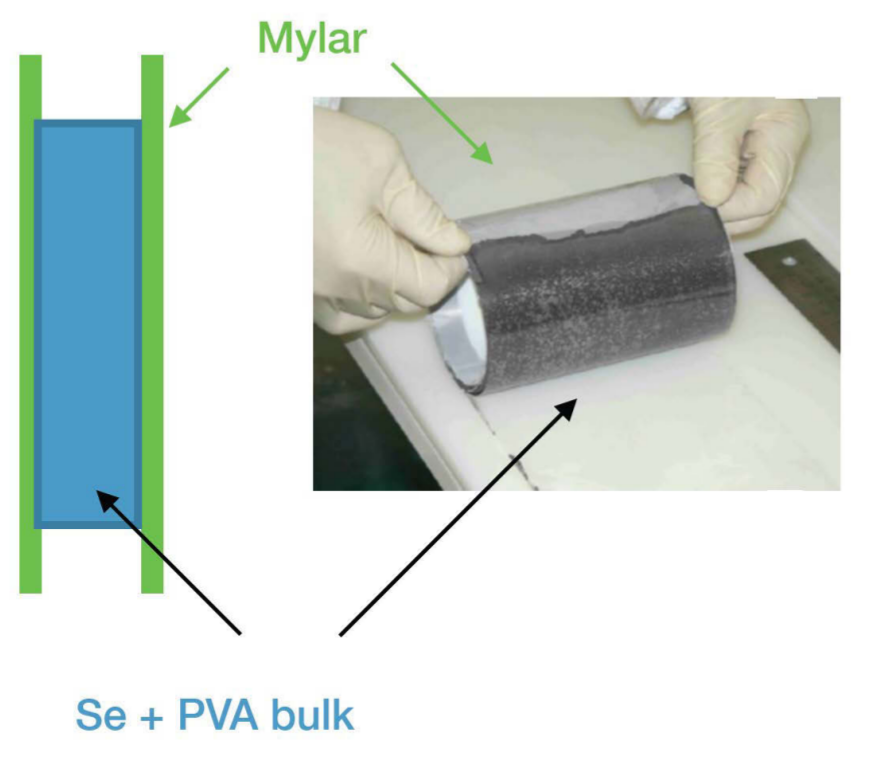
\includegraphics[scale=0.2]{pictures/Chap4/MylarDesign.png}
\caption{Schematic side view of the mylar design.}
\label{MylarDesign}
\end{figure}


\FloatBarrier


\subsubsection{TULLE}


\NI The TULLE design is new design for the source foils in which the $^{\text{82}}$Se and the PVA paste is spread as uniform as possible over a thin layer of bobbinet tulle made of nylon6-6 providing a ligth and resistant mechanical support. A schematic view of the foil design is shown in Figure~\ref{TulleDesign}. The bobbinet tulle is constructed by warp and weft yarns in which the weft yarn is looped diagonally around the vertical warp yarn to form a hexagonal mesh which is regular and clearly defined. To minimise the contamination in $^{\text{208}}$Tl and $^{\text{214}}$Bi coming from the tulle, the lightest fabric available on the market has been chosen, corresponding to a weight of 0.7 mg/cm$^\text{2}$ and was not treated with resins nor paint after waving. The tulle is lighest than the mylar backing film and give the advantage to introduce a smaller contamination of $^{\text{208}}$Tl and $^{\text{214}}$Bi which will translate in lower background levels. Nevertheless, in this design, due to the lack of external protection the source foil is directly in contact with the gas in the tracker and is exposed to the risk of $^{\text{82}}$Se losses. In order to avoid this problem the amount of PVA can be increased to improve the foil strength. An increase of the amount of PVA will translate by an higher contamination and by a higher thickness of the source foil. 


\begin{figure}[h!]
\centering
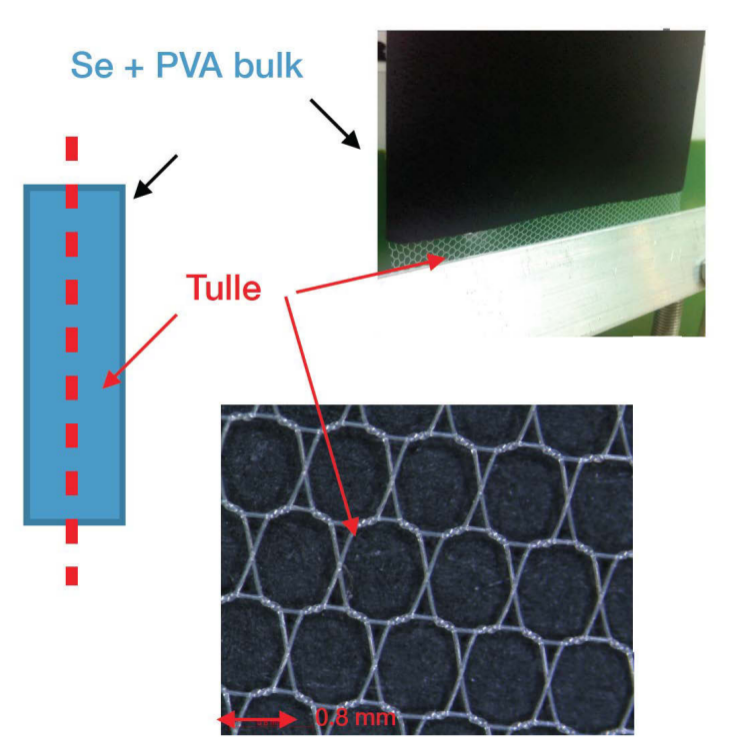
\includegraphics[scale=0.2]{pictures/Chap4/TulleDesign.png}
\caption{Schematic side view of the tulle design.}
\label{TulleDesign}
\end{figure}


\subsection{Discussion}


\NI The parameters used for the modelisation of the source foils for the different designs ares ummarized in Table~\ref{Tab:SummaryParametersSourceFoilDesign} and~\ref{Tab:ExpectedBkgSourceFoilDesign}. In case of the MYLAR foil, which is consedered as an IDEAL foil with two external backing films, the parameters are shown separately for the bulk (b) and the film (f). The TULLE foil is modelled as an IDEAL foil with the nylon mesh uniformly distributed in the foil.


\bigskip


\NI As shown in Table~\ref{Tab:ExpectedBkgSourceFoilDesign}, from the radio-purity point of view, the TULLE design is very promising. Compared to the MYLAR design, even if more PVA is used, it allows to obtain a total activity in $^{\text{214}}$Bi and $^{\text{208}}$Tl which is respectively 18\% and 29\% lower. 



\begin{table}[h!]
\centering
\begin{tabular}{c|c|c|c|c|c|c}
\multirow{2}{*}{Design} & f$_\text{Se}$ & f$_\text{PVA}$ & f$_\text{Support}$ & a                  & $\rho$            & t \\
                        & [-]           & [-]            & [-]                & [mg/cm$^\text{2}$] & [g/cm$^\text{3}$] & [$\mu$m] \\[0.1cm]
\toprule
IDEAL & 0.95  & 0.05 & 0.00  & 52.5                             & 3.11 & 169 \\[0.1cm]
TULLE & 0.888 & 0.10 & 0.012 & 56.3                             & 2.98 & 189 \\[0.1cm]
MYLAR & 0.95  & 0.05 & -     & 52.5$_\text{b}$ + 3.2$_\text{f}$ & 3.11$_\text{b}$ + 1.4$_\text{f}$ & 169$_\text{b}$ + 24$_\text{f}$ \\[0.1cm]
\bottomrule
\end{tabular}
\caption{Summary of the foil parameters for the source foil designs under consideration. The MYLAR design is considered as IDEAL with two external backing films. The parameters in this case are then shown separately for the bulk (b) and the film (f).}
\label{Tab:SummaryParametersSourceFoilDesign}
\end{table}



\begin{table}[h!]
\centering
\begin{tabular}{c|c|c|c|c|c}
\multirow{2}{*}{Design} & f$_\text{Se}$/f$_\text{Se}$ & f$_\text{PVA}$/f$_\text{Se}$ & f$_\text{Support}$/f$_\text{Se}$ & A ($^{\text{214}}$Bi) & A ($^{\text{214}}$Bi)  \\
& [-]   & [-]   & [-]   & [$\mu$Bq/kg] & [$\mu$Bq/kg] \\[0.1cm]
\toprule
IDEAL & 1 & 0.053 & 0.000 & 62.0                               & 3.4   \\[0.1cm]
TULLE & 1 & 0.113 & 0.014 & 142.5                              & 13.5  \\[0.1cm]
MYLAR & 1 & 0.053 & 0.068 & 62.0$_\text{b}$ + 111.6$_\text{f}$ & 3.4$_\text{b}$ + 15.6$_\text{f}$  \\[0.1cm]
\bottomrule
\end{tabular}
\caption{Expected 208 Tl and 214 Bi activities computed from~Equation~\ref{eq:ActivityComponent}. The values do not include the activity of the 82 Se which is not known at this stage.}
\label{Tab:ExpectedBkgSourceFoilDesign}
\end{table}


\FloatBarrier


\section{Monte-Carlo simulations}\label{sec:MCsimulations}


\NI The study performed in this work is based on the event simulation performed through the Falaise-legacy framework. Through a set of configuration files, the user can specify the detector model to be considered (i.e. geometry and materials) and simulate the initial kinematic for different type of events in specific region of the detector (e.g. the source foil). The propaga- tion of the particles through the detector is performed by a GEANT4 based module which simulates all relevant processes, such as multiple scattering, ionisation, Compton scattering, bremsstrahlung. The detector response is then obtained by smearing the true information provided by GEANT4 with respect to the calorimeter and the tracker resolution. Dedicated reconstruction and selection module allow to select events in a specific channel for dedicated analysis.


\bigskip


\NI This work is not meant to document and validate the Falaise-legacy chain, a complete validation of the framework should be found elsewhere. The description available in the following focuses only on the parts relevant for this work. Moreover, the Falaise-legacy is likely to be abandoned in favour of a new version of the framework which is currently under validation. The new software should be used in the future to cross-check the MC production used for this work.


\subsection{Source foils modelisation}


\NI The modelisation of the source foil strips is realized through rectangular boxes made of $^{\text{82}}$Se, PVA, nylon or mylar according from the design under consideration. The composition of the different design introduced in Section~\ref{sec:designUnderConsideration} are used as well as the parameters summarised in Table~\ref{Tab:SummaryParametersSourceFoilDesign}. The implementation of the material composition is performed by defining the fraction mass for each element, mainly $^{\text{82}}$Se, $^{\text{Nat}}$Se, O, C and N which is found in the nylon mesh.


\subsection{Events generation}


\NI The generation of the events is performed uniformly from the source foil. They are generated for the 0$\nu\beta\beta$, 2$\nu\beta\beta$ and the internal background coming from contamination in $^{\text{208}}$Tl and $^{\text{214}}$Bi. For the MYLAR design, to take into account the contamination coming from the backing film, events of $^{\text{208}}$Tl and $^{\text{214}}$Bi are also generated in the mylar film. Table~\ref{Tab:GeneratedEventSource} shows the statistic generated for each event type. 


\begin{table}[h!]
\centering
\begin{tabular}{c|c|c|c|c}
Design & 0$\nu\beta\beta$ & 2$\nu\beta\beta$ & $^{\text{208}}$Tl & $^{\text{214}}$Bi  \\[0.1cm]
\toprule
IDEAL & 10$^{\text{6}}$ & 10$^{\text{7}}$ & 10$^{\text{7}}$ & 10$^{\text{7}}$  \\[0.02cm]
TULLE & 10$^{\text{6}}$ & 10$^{\text{7}}$ & 10$^{\text{7}}$ & 10$^{\text{7}}$  \\[0.02cm]
MYLAR &                 &                 &                 &                  \\[0.02cm]
(bulk)& 10$^{\text{6}}$ & 10$^{\text{7}}$ & 10$^{\text{7}}$ & 10$^{\text{7}}$  \\[0.02cm]
(film)&                 &                 & 10$^{\text{7}}$ & 10$^{\text{7}}$  \\[0.02cm]
\bottomrule
\end{tabular}
\caption{Generated statistics for each event type and source foil design.}
\label{Tab:GeneratedEventSource}
\end{table}


\NI Since the event generation has been performed with many different configurations of the source foil, the statistics has been optimised to contain the event production within reasonable processing time (24 hours).  This current production allows to keep the statistical uncertainty on the number of events selected in the relevant energy region within 0.2\% for the 0$\nu\beta\beta$ and the 2$\nu\beta\beta$ events and within 5\% for the 208 Tl and 214 Bi events which is already a factor 2 lower than the systematic uncertainties observed for the internal background in NEMO-3 (10\%). As these systematics are expected to be similar in SuperNEMO, we consider that the statistics of the MC samples is enough in this contest.


\subsection{Events energy distribution}


\NI The reconstruction of the events and the selection of the 2e channel is then performed. Only the events having two negative tracks hitting two calorimeter blocks with a total energy deposition E $\beta\beta$ > 2 MeV are selected. The energy distributions for the signal and the backgrounds are shown in Figure~\ref{Distribution2eSelection}. These p.d.f will be used therafter to compare among different designs of the source foil. The IDEAL design is shown in black, the TULLE design in red and the MYLAR design in blue. From these distributions it can be seen that the shape of the energy distribution do not depend heavily of the considered design event if a small overall decrease of the event selection efficiency is observed for the TULLE and MYLAR design compared to the IDEAL case. This decrease is more important for the 0$\nu\beta\beta$ and 2$\nu\beta\beta$ while it is not significant for the $^{\text{208}}$Tl and $^{\text{214}}$Bi. The effect is due to the increased thickness of the source foil in the TULLE and the MYLAR designs compared to the IDEAL case, which slightly shifts the p.d.f to the lower energies due to an increased energy loss in the foil. The selection efficiency for the signal and the background obtained in the [2000; 3200] keV energy window are shown in Table~\ref{Tab:EventSelectionEfficiency}.


\begin{figure}[h!]
\centering
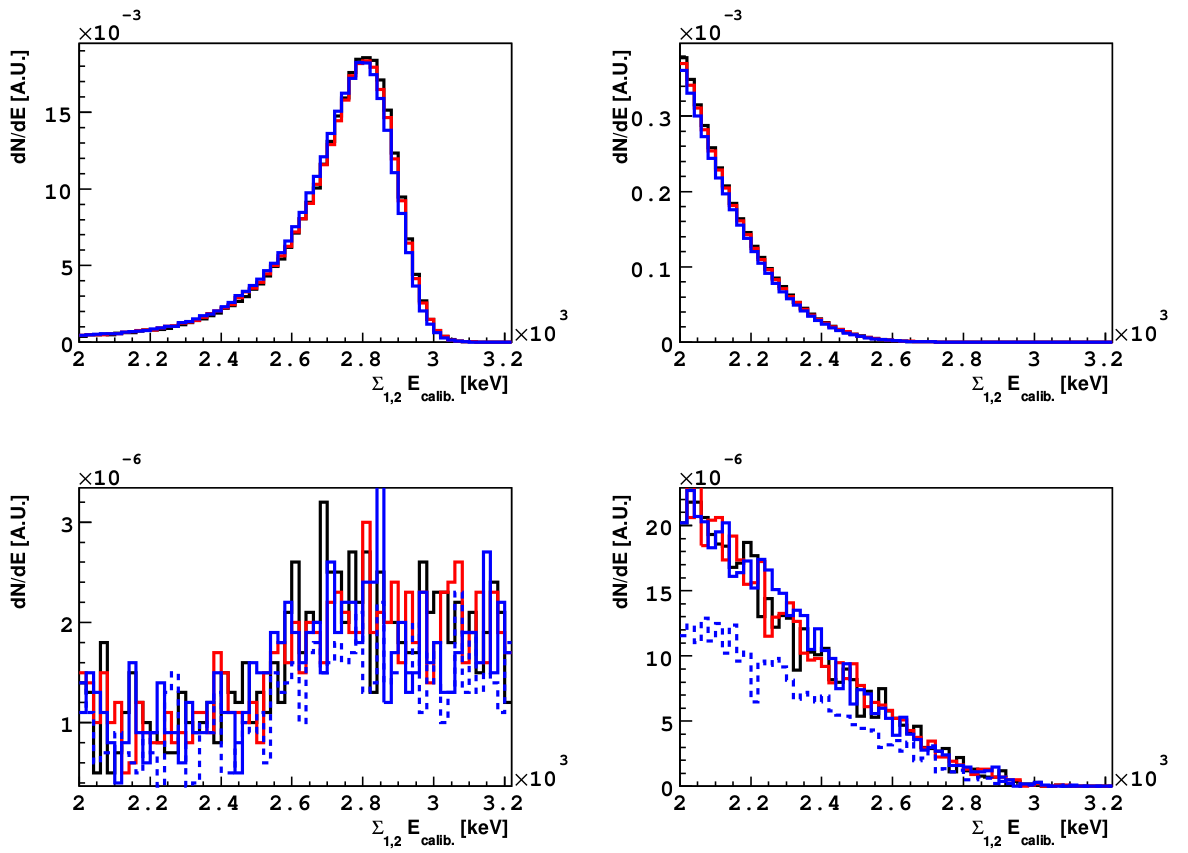
\includegraphics[scale=0.24]{pictures/Chap4/Distribution2eSelection.png}
\caption{Comparaison of the 2e energy distribution for signal and background channels for different design of the source foil. Black IDEAL. Red : TULLE. Blue : MYLAR. Top left : 0$\nu\beta\beta$, top right : 2$\nu\beta\beta$, bottom left : 208Tl, bottom right : Bi214. The dashed blue histogram in the bottom plots represent the expected energy for events generated in the mylar backing film.}
\label{Distribution2eSelection}
\end{figure}


\begin{table}[h!]
\centering
\begin{tabular}{c|c|c|c|c}
\multirow{2}{*}{Design} & $\epsilon_{\text{0}\nu}$ & $\epsilon_{\text{2}\nu}$ & $\epsilon_{\text{Tl}}$ & $\epsilon_{\text{Bi}}$  \\
& [\%]   & $\times$ 10$^{-\text{2}}$ [\%] & $\times$ 10$^{-\text{2}}$ [\%] & $\times$ 10$^{-\text{2}}$ [\%] \\[0.1cm]
\toprule
IDEAL & 29.01 $\pm$ 0.05 & 33.64 $\pm$ 0.04 & 0.99 $\pm$ 0.03 & 4.3 $\pm$ 0.1 \\[0.05cm]
\hline
TULLE & 28.84 $\pm$ 0.04 & 33.05 $\pm$ 0.04 & 0.95 $\pm$ 0.03 & 4.4 $\pm$ 0.1 \\[0.05cm]
\hline
MYLAR & & & & \\[0.1cm]
(bulk)& 28.86 $\pm$ 0.04 & 31.75 $\pm$ 0.04 & 0.92 $\pm$ 0.03 & 4.5 $\pm$ 0.1 \\[0.05cm]
(film)& & & 0.73 $\pm$ 0.03 & 2.7 $\pm$ 0.1 \\ 
\bottomrule
\end{tabular}
\caption{Event selection efficiency in the 2e channel in [2000; 3200] keV.}
\label{Tab:EventSelectionEfficiency}
\end{table}


\FloatBarrier


\section{Sensitivity study}\label{sec:SensStudy}


\NI The study of the sensitivity of an experiment looking for a new phenomena, allows to estimate its physics case and compare among different competing experiments. During the designing phase, it is also useful to study the sensitivity with respect to different detector configurations in order to find the optimal design.


\bigskip


\NI In order to define the sensitivity to a phenomena not yet observed, we assume the experiment does not observe any signal. In this worse case scenario, we study which portion of the allowed parameter phase space the experiment can exclude.


\bigskip


\NI In the following sections, different methods to compute SuperNEMO sensitivity are described in details. The sens software package, which implements each sensitivity computation method, is also described. This section serves as reference manual for the user. The p.d.fs obtained in the previous chapter with the IDEAL design are used in the following as example of sensitivity computation. Here the backgrounds are normalised to 2 $\mu$Bq/kg and 10 $\mu$Bq/kg for the 208 Tl and the 214 Bi internal background respectively (i.e. the target radio-purity level of SuperNEMO). The 2$\nu\beta\beta$ background is normalised to 9 $\times$ 10 19 y as measured in NEMO-3 [7]. This configuration is referred in the text as IDEAL (star).



\subsection{R.O.I method}


\NI As defined in Section~\ref{sec:ExperimentalSearch0nu}, the sensitivity on the 0$\nu\beta\beta$ decay half-life is given by~:


\begin{equation}
\text{T}_{\text{1/2}}^{\text{0}\nu} > \frac{\text{N}_\text{A}~\text{ln2}}{\text{W}} \times \frac{\epsilon \times \text{M} \times \text{T}}{\mathcal{S}(\text{b})}
\end{equation}


\NI where N$_\text{A}$ is the Avogadro number, W the atomic mass of the $\beta\beta$ isotope under study, $\epsilon$ is the signal selection efficiency and M $\times$ T the total experimental exposure. The $\mathcal{S}$(b)term represents the average upper limit on the number of signal events that would be obtained by an ensemble of identical replicas of such experiment, each one with the same mean expected background and no true signal. The Feldman \& Cousins unified approach for the definition of the confidence level is adopted. This method optimises the region of interest (R.O.I.) with respect to the sensitivity to the T$_{\text{1/2}}^{\text{0}\nu}$. This optimisation is achieved by maximising the $\epsilon$/S(b) ratio for a given exposure M~$\times$~T.


\subsection{Selection efficiency}


\NI The signal and the background selection efficiencies in the 2e channel are obtained integrating the respective p.d.f.


\begin{equation}
\epsilon_\text{i} (\text{E}_{\text{low}};\text{E}_{\text{up}}) = \frac{1}{\text{N}} \int_{\text{E}_{\text{low}}}^{\text{E}_{\text{up}}} \frac{\text{dN}}{\text{dE}} \text{dE}
\end{equation}


\bigskip 


\NI Where the energy interval (E Low ; E Up ) define the R.O.I.. The plot in fig. 4.1 show the value of efficiency for the 0$\nu\beta\beta$ signal (red) and background (2$\nu\beta\beta$ in blue, 214 Bi in yellow and 208 Tl in green) when the upper edge of the R.O.I. is kept fix at 4500 keV while the lower edge is moved from 2000 keV up to 3500 keV.


\bigskip


\NI Those efficiencies are then used to estimate the expected background level for a given exposure M $\times$ T following :


\begin{equation}
\text{N}_{\text{2}\nu} = \frac{\text{N}_\text{A}~\text{ln2}}{\text{W}} \times \frac{\epsilon_{\text{2}\nu} \times \text{M} \times \text{T}}{\text{T}_{\text{1/2}}^{\text{2}\nu}}
\end{equation}


\begin{equation}
\text{N} (^{\text{214}}\text{Bi}) = \text{A} (^{\text{214}}\text{Bi}) \times \epsilon (^{\text{214}}\text{Bi}) \times \text{M} \times \text{T} 
\end{equation}


\begin{equation}
\text{N} (^{\text{208}}\text{Tl}) = \text{A} (^{\text{208}}\text{Tl}) \times \epsilon (^{\text{208}}\text{Tl}) \times \text{M} \times \text{T} 
\end{equation}


\NI Where T 1/2 Is the measured half-life for the 2$\nu\beta\beta$ decay while A214Bi and 208 A 208Tl are the expected activity level of Bi and Tl contamination of the foil source. The renormalisation of the histogram in fig. 4.1 through eq. 4.3, 4.4 and 4.5 provide the expected number of background events as a function of the low energy edge of the R.O.I. as shown in fig. 4.2.


\bigskip


\NI The integral of eq. 4.2 can also be computed changing both edges of the R.O.I. obtaining a 2D scan of the selection efficiencies. The same renormalisation through eq. 4.3, 4.4 and 4.5 provide the 2D scan of the expected number of background events w.r.t. the edges of the R.O.I. as shown in fig. 4.3.

\begin{figure}[h!]
\centering
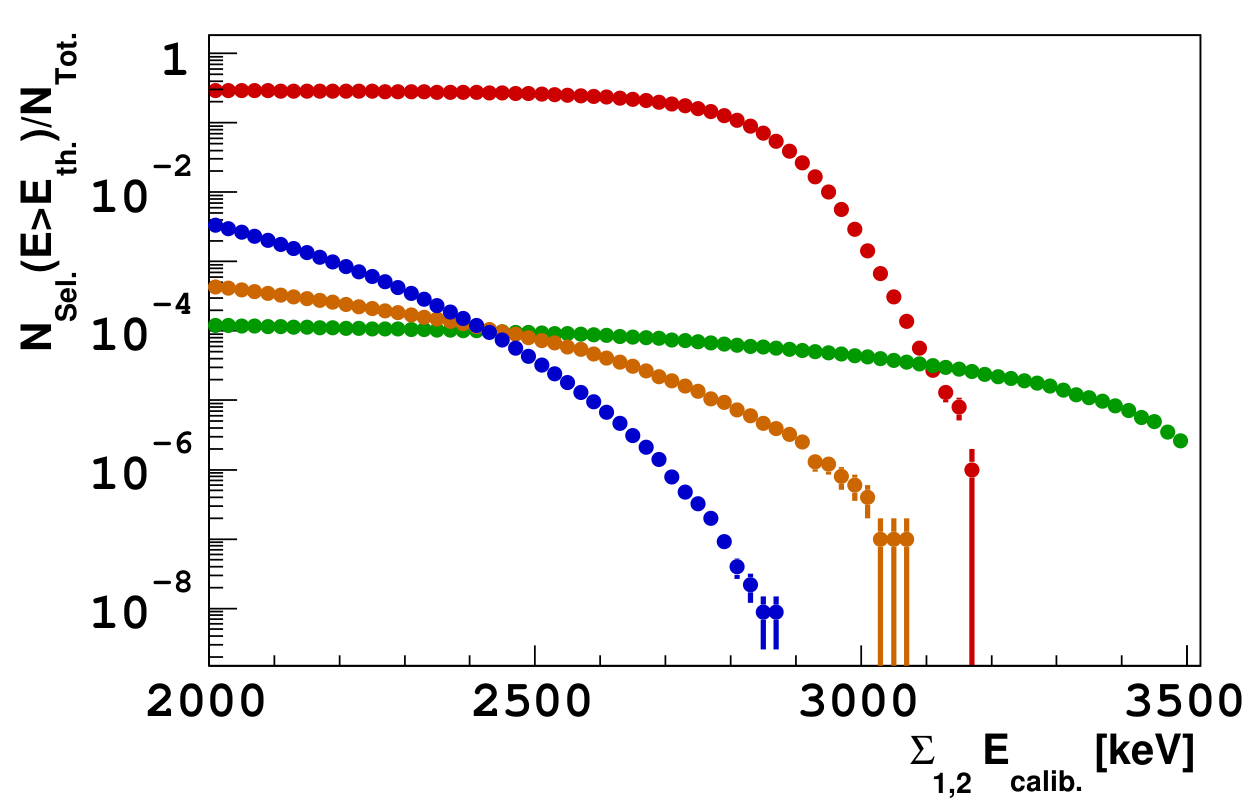
\includegraphics[scale=0.25]{pictures/Chap4/SelectionEfficiency.png}
\label{SelectionEfficiency.png}
\caption{Selection efficiency for the 0$\nu\beta\beta$ signal (red) and the different backgrounds (2$\nu\beta\beta$ in blue, Bi214 in yellow and Tl208 in green). The upper edge of the R.O.I is kept fix at 4500~keV while the lower edge is moved from 2000~keV up to 3500~keV.}
\end{figure}


\begin{figure}[h!]
\centering
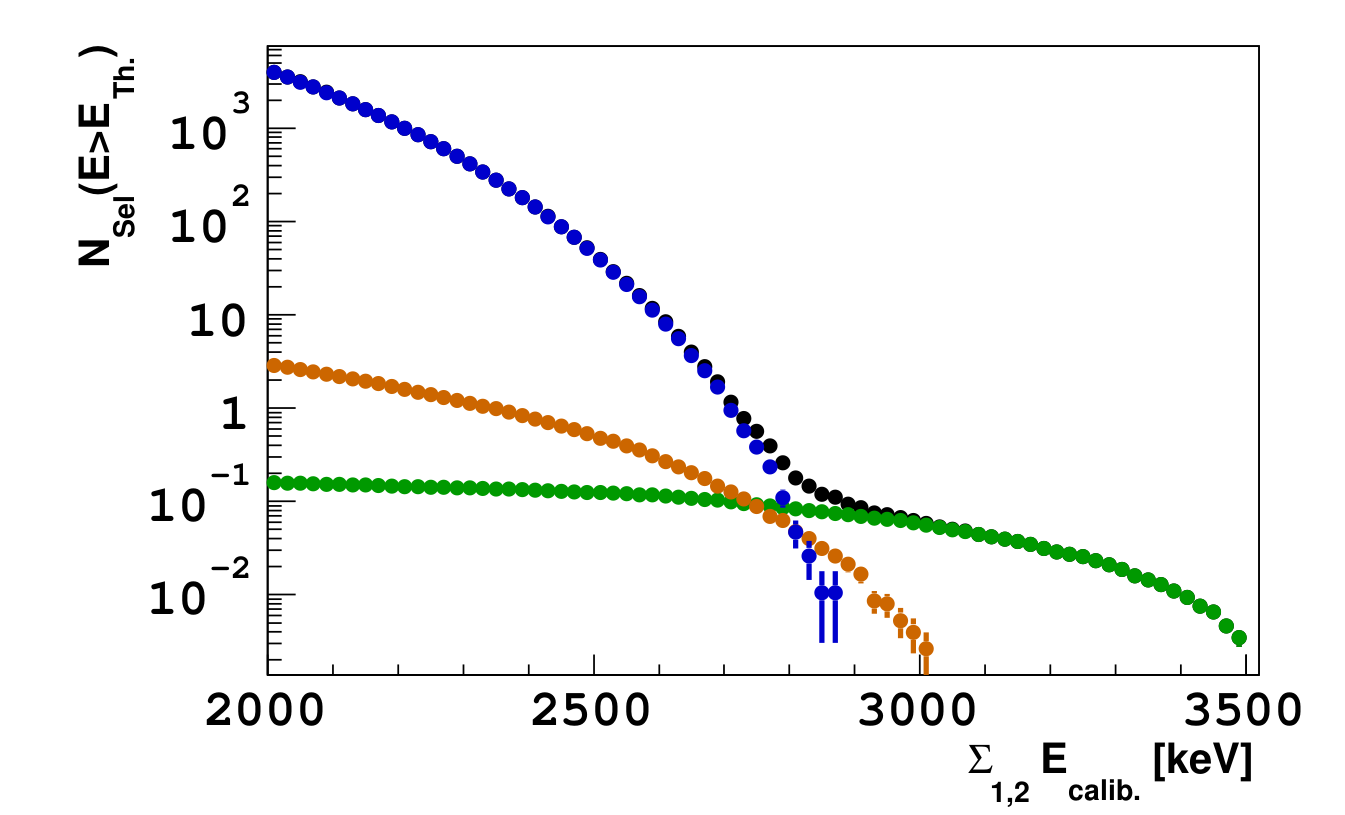
\includegraphics[scale=0.25]{pictures/Chap4/ExpectedNumberofEvent.png}
\label{ExpectedNumberofEvent.png}
\caption{Expected number of background events (2$\nu\beta\beta$ in blue, Bi214 in yellow and Tl208 in green) as a function of the low energy edge of the R.O.I. The black points show the sum of all background contributions.}
\end{figure}


\begin{figure}[h!]
\centering
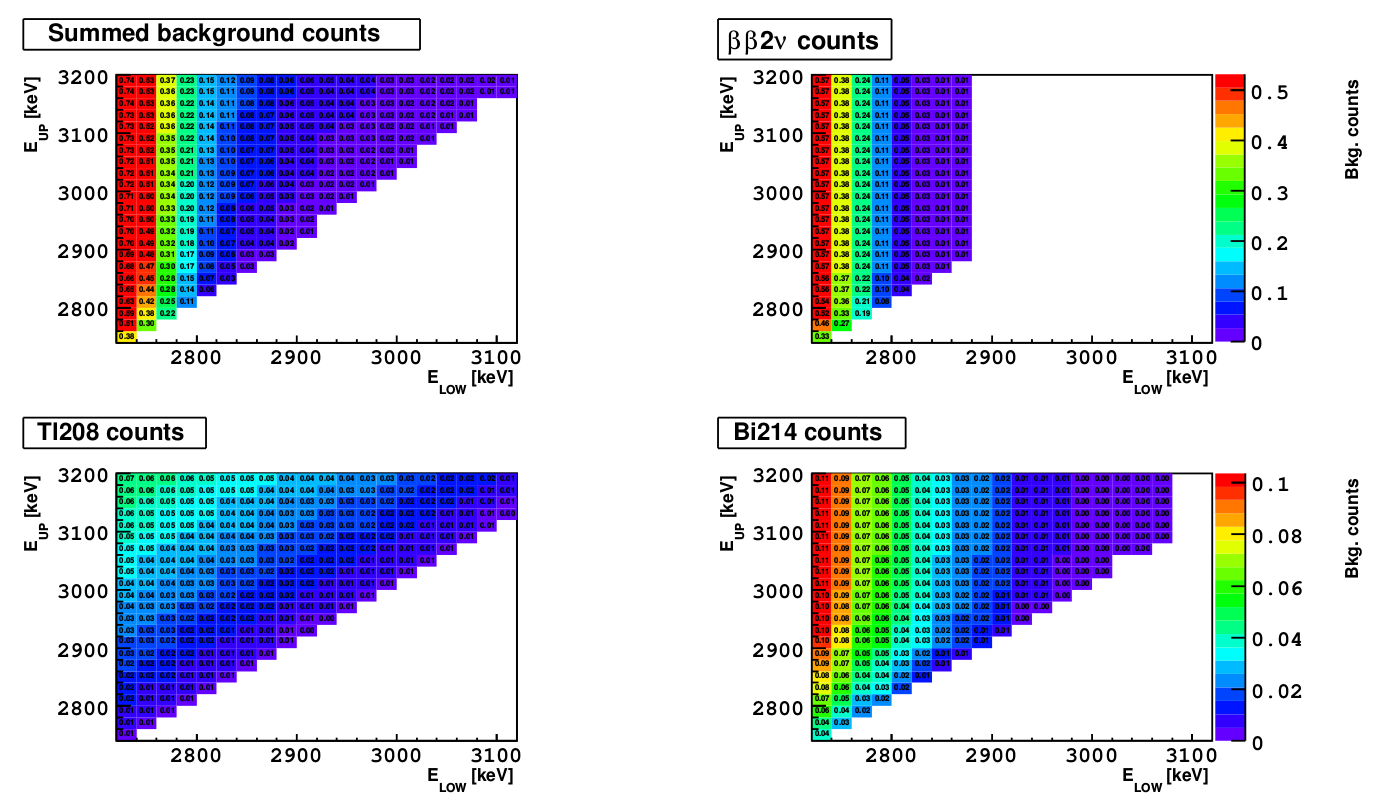
\includegraphics[scale=0.4,  angle =90]{pictures/Chap4/BkgCount2D.png}
\label{BkgCount2D.png}
\caption{Expected background counts as a function of the edges of the R.O.I..}
\end{figure}


\FloatBarrier


\subsection{The Feldman \& Cousins 90\% C.L.}
 

\NI The term S(b) of eq. 4.1 is defined following the Feldman \& Cousins prescription for the definition of confidence interval of small signal [8]. Defining U(n$|$b) as the function yielding the (unified approach) upper limit (at the desired C.L.) for a given observation n and a mean predicted background level b. Values for U(n$|$b) are reported in tabular form in [?] for several C.L. values. Given that the variable n follows a Poisson p.d.f., P(n$|$b) = P(n; b), then S(b) is given by : 


\begin{equation}
\mathcal{S}(b) = \text{E}[\mathcal{U}(n|b)] = \sum_{n=0}^{\infty} \mathcal{P} (n;b) \times \mathcal{U}(n|b)
\end{equation}


\NI The sensitivity S(b) of an experiment expecting b events of background and no true signal is obtained by averaging the upper limits obtained using the unified approach U(n$|$b) with the likelihood of the individual observations P(n$|$b). The fig. 4.4 shows the 90\% C.L. curve for a background level spanning in [0; 40] c.t.s. It must be noticed that in the large background approximation, the sensitivity curve as a function of b follows the expected classical limit obtained through the Neyman construction of the confidence belt :


\begin{equation}
\mathcal{S}(b) \propto a \times \sqrt{b}, ~\text{for}~\text{large}~\text{b} 	
\end{equation}


\bigskip


\NI where a =1.64 (1.96) at 90\% (95\%) CL.


\begin{figure}[h!]
\centering
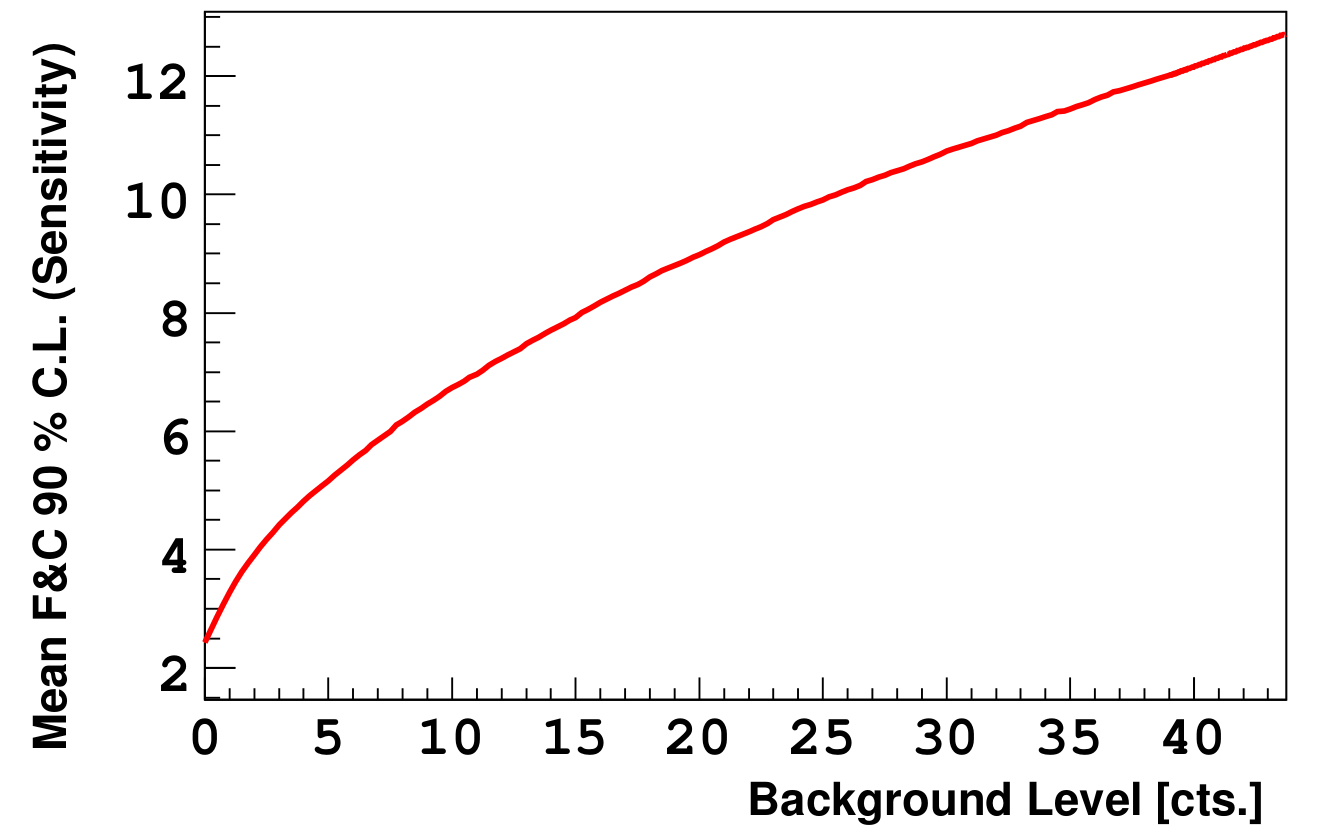
\includegraphics[scale=0.22]{pictures/Chap4/FeldmanAndCousin.png}
\label{FeldmanAndCousin.png}
\caption{The 90\% C.L. sensitivity curve as a function of the number of background events.}
\end{figure}


\FloatBarrier


\subsection{1d vs 2d R.O.I. optimisation}


\NI Computing the sensitivity from eq. 4.1 as a function of the R.O.I. for a given experimental exposure define the best sensitivity of the experiment. The plot in fig. 4.5 show the 1d sensitivity scan as a function of the low energy edge of the R.O.I.. The high energy edge is kept fix at 3200 keV. The best sensitivity of 6.1$\times$10 24 y is found in [2720; 3200] keV after 21 kg$\times$y exposure, with an expected total background contamination of 0.74 $\pm$ 0.06 cts. in the R.O.I..


\begin{figure}[h!]
\centering
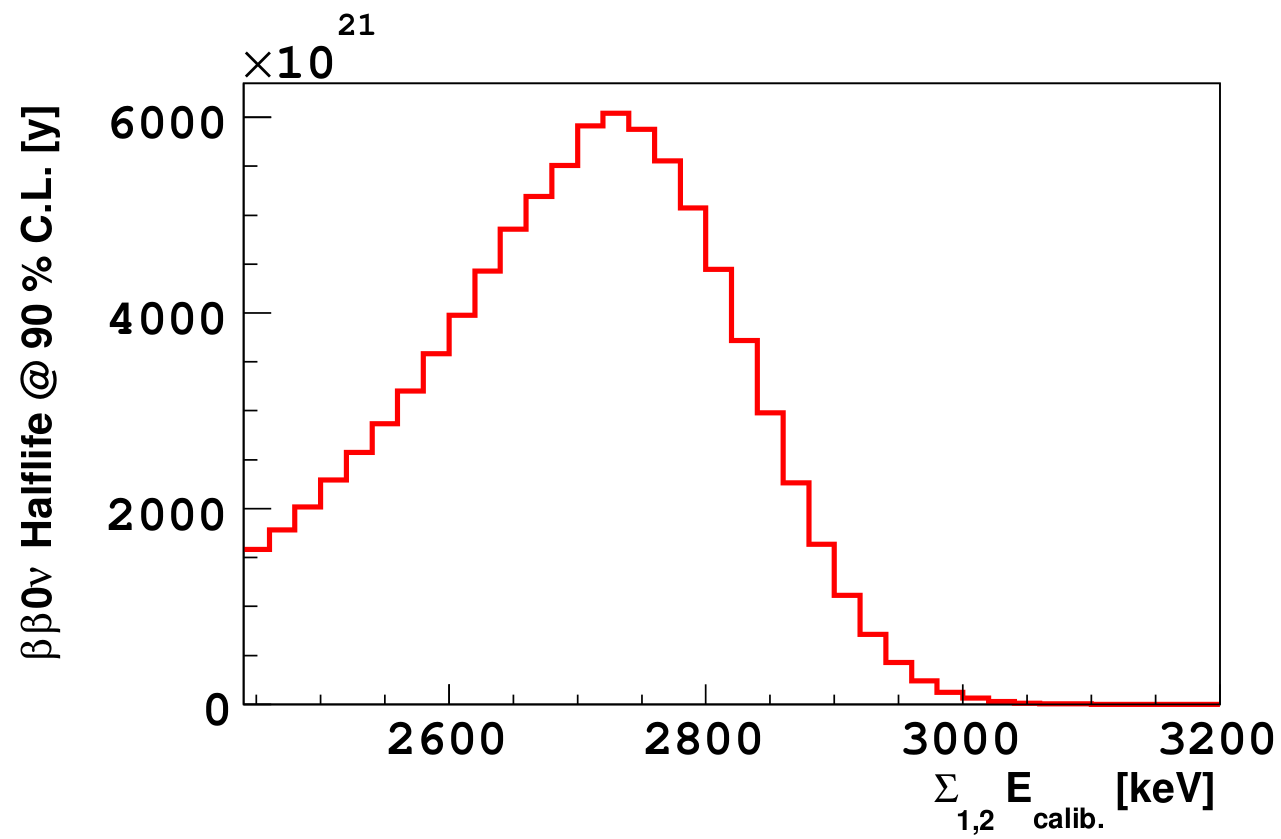
\includegraphics[scale=0.25]{pictures/Chap4/Sens0nu1D.png}
\label{Sens0nu1D.png}
\caption{The 1d sensitivity scan as a function of the low energy edge of the R.O.I.. The high energy edge is kept fix at 3200 keV. The best sensitivity of 6.1 $\times$ 10 24 y is found in [2720; 3200] keV after 21 kg$\times$y exposure, with an
expected total background contamination of 0.74 $\pm$ 0.06 cts.}
\end{figure}


\bigskip

\NI Since the decay chain of the 208 Tl has an high energy gamma, the expected 2e energy spectral shape extend at high energy up to 3500 keV, above the end point of the $\beta\beta$ energy spectrum of the 82 Se at Q $\beta\beta$ = 2995 keV as shown in fig. 4.2. In order to minimise such background contamination, the simultaneous optimisation of the two edges of the R.O.I. is performed in fig. 4.6. The best sensitivity of 6.12 $\times$ 10 24 y is found in [2720; 3060] keV after 21 kg$\times$y exposure, with an expected total background contamination of 0.72 $\pm$ 0.06 cts. in the R.O.I.. No major reduction of the background is observed, the results are found to be compatible within the statistical uncertainties.


\begin{figure}[h!]
\centering
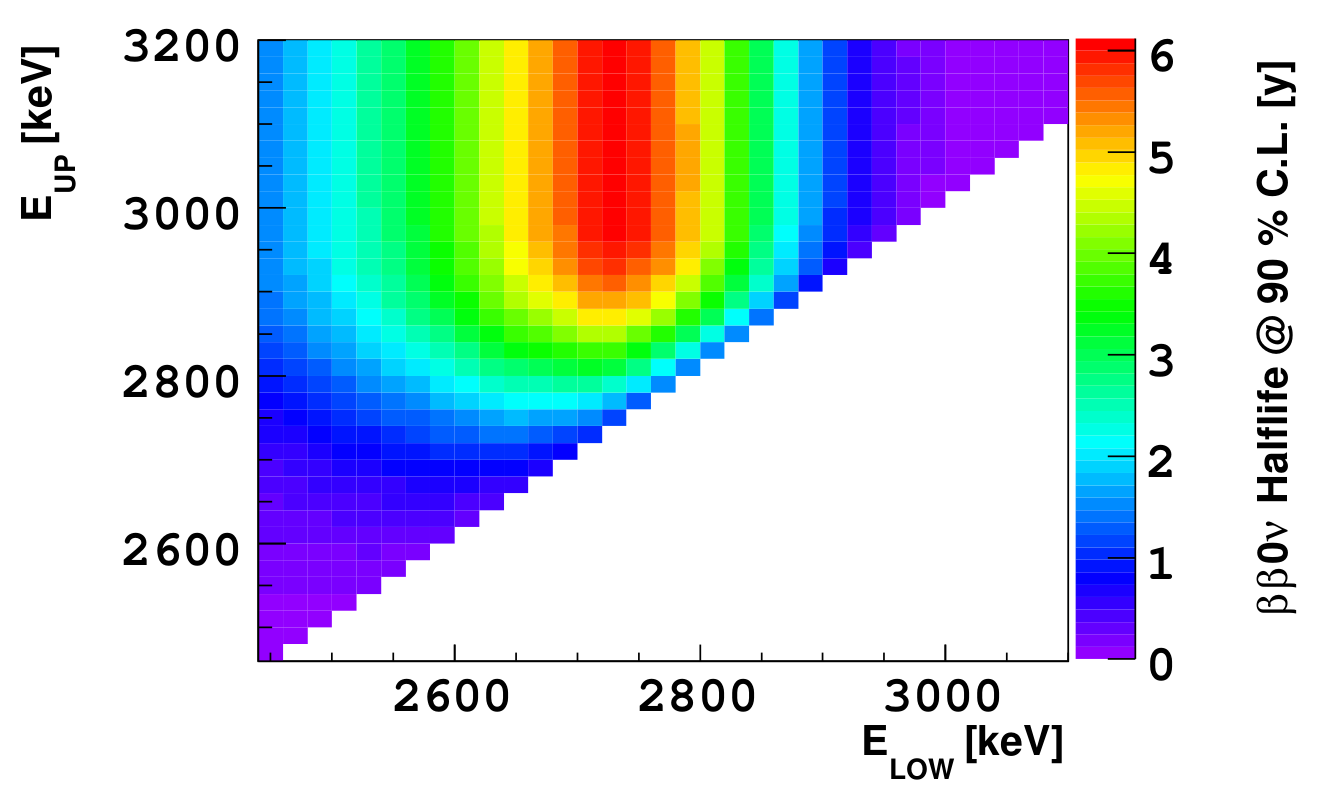
\includegraphics[scale=0.25]{pictures/Chap4/Sens0nu2D.png}
\label{Sens0nu2D.png}
\caption{The 2d sensitivity scan as a function of the energy edges of the R.O.I.. The best sensitivity of 6.12 $\times$ 10 24 y is found in [2720; 3060] keV after 21 kg$\times$y exposure, with an expected total background contamination of 0.72 $\pm$ 0.06 cts.}
\end{figure}


\FloatBarrier


\subsection{Validation of the background level}


\NI As already mentioned, the results of the simulation performed with the Falaise-legacy framework has not been validated in details here. The recent NEMO-3 results on the 100 Mo [6] could be used to crosscheck the background level obtained in sec. 4.1. The eq. 4.3, 4.4 and 4.5 could in fact be used to scale the background measured in NEMO-3 to the target 208 Tl and 214 Bi activities and to the exposure of the SuperNEMO demonstrator.


\bigskip


\NI The values in tab. 4.1 shown the internal 208 Tl and 214 Bi activities measured in NEMO-3, the measured background level in [2.8; 3.2] MeV and its extrapolation to the activities and exposure expected for the SuperNEMO demonstrator. The last column of the table shows the expected background level extracted from fig. 4.3, considering the same R.O.I. as NEMO-3. 


\bigskip


\NI A discrepancies of 33\% and 42\% is observed for the 208 Tl and the 214 Bi respectively. However, it must be kept in mind that a direct comparisons could not apply since NEMO-3 and SuperNEMO are not the same detector. SuperNEMO in fact has a better energy resolution (8\% at 1 MeV w.r.t. the 14\% of NEMO-3) and an higher detection efficiency due to an optimised design of the tracker and the calorimeter. While NEMO-3 has a 0$\nu\beta\beta$ detection efficiency of 4.7\% in [2.8; 3.2] MeV, for SuperNEMO this value is 11\%, as obtained from the simulation performed in this work. Neglecting the different energy resolution (208 Tl and 214 Bi spectra are rather flat in the R.O.I.) the values of tab. 4.1 agrees within 20\% when considering that the 0$\nu\beta\beta$ selection efficiency of SuperNEMO is $\times$ 2.3 higher than NEMO-3.


\subsection{Validation of the sensitivity calculation}


\NI The sensitivity value obtained with the extended likelihood method in sec. 4.2 could be compared to the results obtained in [1], since the method is the same. The plot in fig. 4.8 shown the T 1/2 an exposure of 500 kg$\times$y as a function of the calorimeter energy resolution obtained in [1]. The dependence of the thickness of the source foil is also shown with different colour. The internal background activities have been set to 2 $\mu$Bq/kg and 10 $\mu$Bq/kg for 208 Tl and 214 Bi respectively.


\bigskip


\NI Even if the design of the detector adopted in [1] is slightly different to the final one being considered in this work, a qualitative comparisons could be performed choosing the values corresponding to the current detector parameters. The final detector design adopted in this work consider a calorimeter resolution of 8\% FWHM at 1 MeV and a source foil thickness of 50 mg/cm 2 . The relevant sensitivity value from fig. 4.8 is then between 7.5 $\times$ 10 25 y and 9.5 $\times$ 10 25 y corresponding to a thickness of 40 mg/cm 2 and 60 mg/cm 2 respectively.


\bigskip


\NI The extrapolation of the calculation performed in the previous section up to 500 kg$\times$y results in a sensitivity of 8.3 $\times$ 10 25 y at 90\% C.L which agrees within 12\% with the values obtained in [1]. The agreements improve to 3.5\% when the 208 Tl and 214 Bi internal backgrounds are neglected.


\begin{table}
\centering
\begin{tabular}{c|cc|cc|c}
                  & \multicolumn{2}{c|}{NEMO-3}                      & \multicolumn{2}{c|}{Extrapolation} & Expectation \\
                  & \multicolumn{2}{c|}{($^{\text{100}}$Mo results)} & \multicolumn{2}{c|}{(to SuperNEMO)} & (simulation) \\[0.1cm]
\toprule
                  & Activities   & Events           & Activities  & Events            & Events \\  
                  & [$\mu$Bq/kg] & in 22 kg$\times$y& [$\mu$Bq/kg] &in 21 kg$\times$y  & in 21 kg$\times$y\\  [0.1cm]
\hline
$^{\text{208}}$Tl & 128 $\pm$ 3  & 2.39 $\pm$ 0.22 & < 2        & 0.036 $\pm$ 0.004 & 0.054 $\pm$ 0.003 \\
$^{\text{214}}$Bi & 380 $\pm$ 40 & 0.92 $\pm$ 0.13 & < 10       & 0.028 $\pm$ 0.004 & 0.048 $\pm$ 0.006 \\
\bottomrule
\end{tabular}
\caption{The internal 208 Tl and 214 Bi activities measured in NEMO-3, the measured background level in [2.8; 3.2] MeV and its extrapolation to the activities and exposure expected for the SuperNEMO demonstrator. The last column shows the expected background level obtained from the calculation of sec. 4.1, considering the same R.O.I. as NEMO-3.}
\label{Tab:Extrapolation}
\end{table}


\subsection{Estimation of the systematic uncertainty}


\NI The uncertainty on the sensitivity calculation could be roughly estimated assuming the same systematic uncertainties as NEMO-3. The results obtained in [6] quote the following uncertainties in the R.O.I.: $\pm$10\% on the 0$\nu\beta\beta$ selection efficiency $\pm$ 0.7\% on the 2$\nu\beta\beta$ background and $\pm$10\% for both 214 Bi and 208 Tl background. Taking into account those values in the sensitivity calculation with the R.O.I. method, an uncertainty of about $\pm$11\% is obtained on the half-life limit. The worse case scenario in which the signal selection efficiency and the backgrounds fluctuate in opposite directions is assumed for simplicity. The tab. 4.2 summarises the results of the sensitivity scan taking into account the NEMO-3 systematics uncertainties.


\begin{table}
\centering
\begin{tabular}{c|c|c|c|c}
\multicolumn{2}{c|}{Syst. effect} & R.O.I & Bkg. & T$_{\text{1/2}}^{\text{0}\nu}$ \\
$\epsilon_{\text{0}\nu}$ & Bkg. & [keV] & [c.t.s] & [$\times$ 10$^{\text{24}}$~y] \\[0.1cm]
\toprule
-10\%                    & +10\% & [2720;3060] & 0.74 $\pm$ 0.06 & 5.54 \\[0.1cm]
\hline
\multicolumn{2}{c|}{none}   & [2720;3060] & 0.72 $\pm$ 0.06 & 6.12 \\[0.1cm]
\hline
+10\%                    & -10\% &[2720;3060] & 0.71 $\pm$ 0.06 & 6.83 \\[0.1cm]
\bottomrule
\end{tabular}
\caption{Sensitivity scan taking into account the NEMO-3 systematic uncertainties [6]: $\pm$10\% on the 0$\nu\beta\beta$ selection efficiency, $\pm$ 0.7\% on the 2$\nu\beta\beta$ background and $\pm$ 10\% for both 214 Bi and 208 Tl}
\label{Tab:SystUncertaintiesSourceFoil}
\end{table}


\begin{table}
\centering
\begin{tabular}{c|c|c|c}
\toprule
Method & R.O.I [keV] & Bkg. [c.t.s] & T$_{\text{1/2}}^{\text{0}\nu}$ [$\times$ 10$^{\text{24}}$~y] \\[0.1cm]
\hline
R.O.I 1d & [2720 - 3200] & 0.74 $\pm$ 0.06 & 6.09 \\ [0.1cm]
R.O.I 2d & [2720 - 3060] & 0.72 $\pm$ 0.06 & 6.12 \\ [0.1cm]
\bottomrule
\end{tabular}
\caption{Sensitivity calculation methods applied to the IDEAL star design.}
\label{Tab:SensCalculationIDEAL}
\end{table}


\section{Source foil design and detector performance}\label{sec:SourceFoilDesignDetectorPerformance}


\NI The event simulated through the Falaise-legacy software and the method developed in chap.4 to compute the sensitivity are used in the following sections to study the performance of the SuperNEMO detector. The background level and the sensitivity achievable with the different designs of the source foil introduced in chap. 2 are compared in sec. 5.1 and 5.2 respectively. The amount of PVA glue to mix with 82 Se during the production of the TULLE design is optimised in order to provide competitive performance with respect to the alternative MYLAR design in sec. 5.3. Finally the effects of a non uniform thickness of the source foil is evaluated in sec 5.4 providing a target value for the foil production.


\subsection{Radio-purity vs background level}


\NI The different designs of the source foil have an impact on the event selection efficiency in the 2e channel, as highlighted in tab. 3.2 considering events in the [2000; 3200] keV energy region. These differences translate into a different background level for a given internal contamination and a given exposure. Assuming an exposure of 21 kg$\times$y the expected level of background in the optimised R.O.I. is computed changing the 208 Tl and the 214 Bi activity from 0 $\mu$Bq/kg to 15 $\mu$Bq/kg. The resulting histograms are shown in fig. 5.1. The fig. 5.2 shows the amount of internal contamination only, i.e. without the contribution from 0$\nu\beta\beta$ events. It should be noted that for the MYLAR design, each value of activity is equally shared among the p.d.f. of the bulk and the backing film. If all the activity is given to the bulk p.d.f. only, the background increase by 10 . Compatible background level is found as a function of the 208 Tl and 214 Bi activities among the source foil designs. At the target radio-purity level of 2 $\mu$Bq/kg in 208 Tl and 10 $\mu$Bq/kg in 214 Bi the expected background coming from the internal contamination is 0.15 counts for an exposure of 21 kg$\times$y.


\subsection{Sensitivity vs. foil designs}


\NI The values in tab. 5.1 summarise the performance achievable with the SuperNEMO demonstrator module with respect to the source foil design, considering an exposure of 21 kg$\times$y. The signal and the background p.d.f. obtained as described in chap. 3 has been normalised to the 208 Tl and 214 Bi activities measured by BiPo and summarised in tab. 2.3. The label IDEAL star in tab. 5.1 refers, as in chap. 4, to IDEAL design case in which the background p.d.f. are normalised to the target radio-purity level of SuperNEMO. The plots in fig. 5.3 show the result of the sensitivity scan w.r.t. the energy edges of the R.O.I.


\begin{table}
\centering
\begin{tabular}{c|c|c|c|c}
\toprule
Design & R.O.I [keV] & $\epsilon_{\text{0}\nu}$ [\%] & bkg. [cts.] &   T$_{\text{1/2}}^{\text{0}\nu}$ [$\times$ 10$^{\text{24}}$~y] \\[0.1cm]
\hline
IDEAL$^{\star}$ & [2720 ; 3060] & 17.44 $\pm$ 0.04 & 0.7 $\pm$ 0.1 & 6.12 \\  [0.1cm]
\hline
IDEAL           & [2720 ; 3060] & 17.44 $\pm$ 0.04 & 1.3 $\pm$ 0.1 & 5.34 \\  [0.1cm]
\hline
TULLE           & [2720 ; 3020] & 16.98 $\pm$ 0.04 & 2.3 $\pm$ 0.1 & 4.47 \\  [0.1cm]
\hline
MYLAR           & [2720 ; 3000] & 16.44 $\pm$ 0.04 & 2.1 $\pm$ 0.1 & 4.50 \\  [0.1cm]
\bottomrule
\end{tabular}
\caption{SuperNEMO demonstrator performance for different source foil design.}
\label{SNperformanceDiffDesign}
\end{table}


\begin{figure}[h!]
\centering
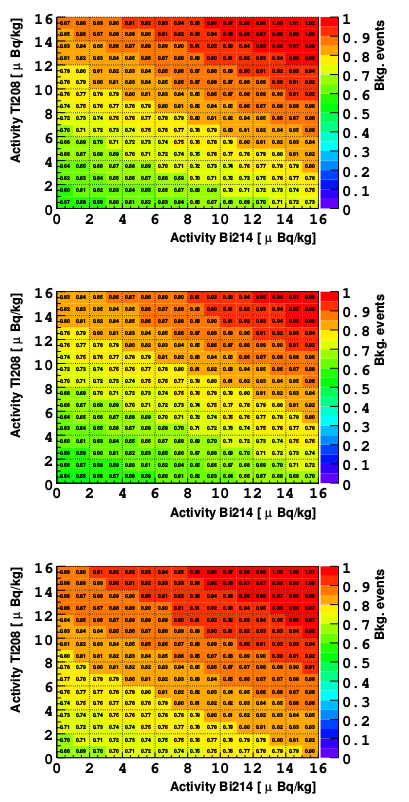
\includegraphics[scale=0.7]{pictures/Chap4/Nbkg_3designs.png}
\label{Nbkg_3designs.png}
\caption{Expected number of total (2$\nu\beta\beta$ + 208 Tl + 214 Bi) background events as a function of the 208 Tl and 214 Bi activity in the source foil for an exposure of 21 kg$\times$y as expected for the SuperNEMO demonstrator. Top: IDEAL. Center: TULLE. Bottom: MYLAR}
\end{figure}


\begin{figure}[h!]
\centering
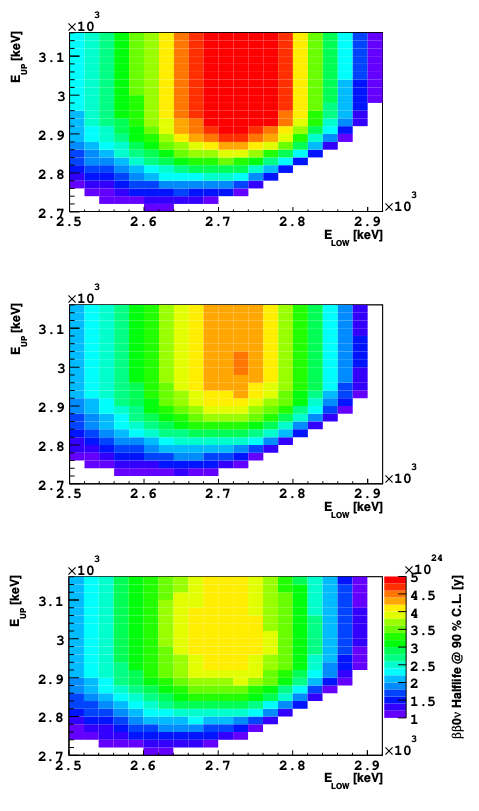
\includegraphics[scale=0.7]{pictures/Chap4/Sens2D-3designs.png}
\label{Sens2D-3designs.png}
\caption{SuperNEMO demonstrator sensitivity for different source foil design. Top: IDEAL. Center: TULLE. Bottom: MYLAR}
\end{figure}


\begin{figure}[h!]
\centering
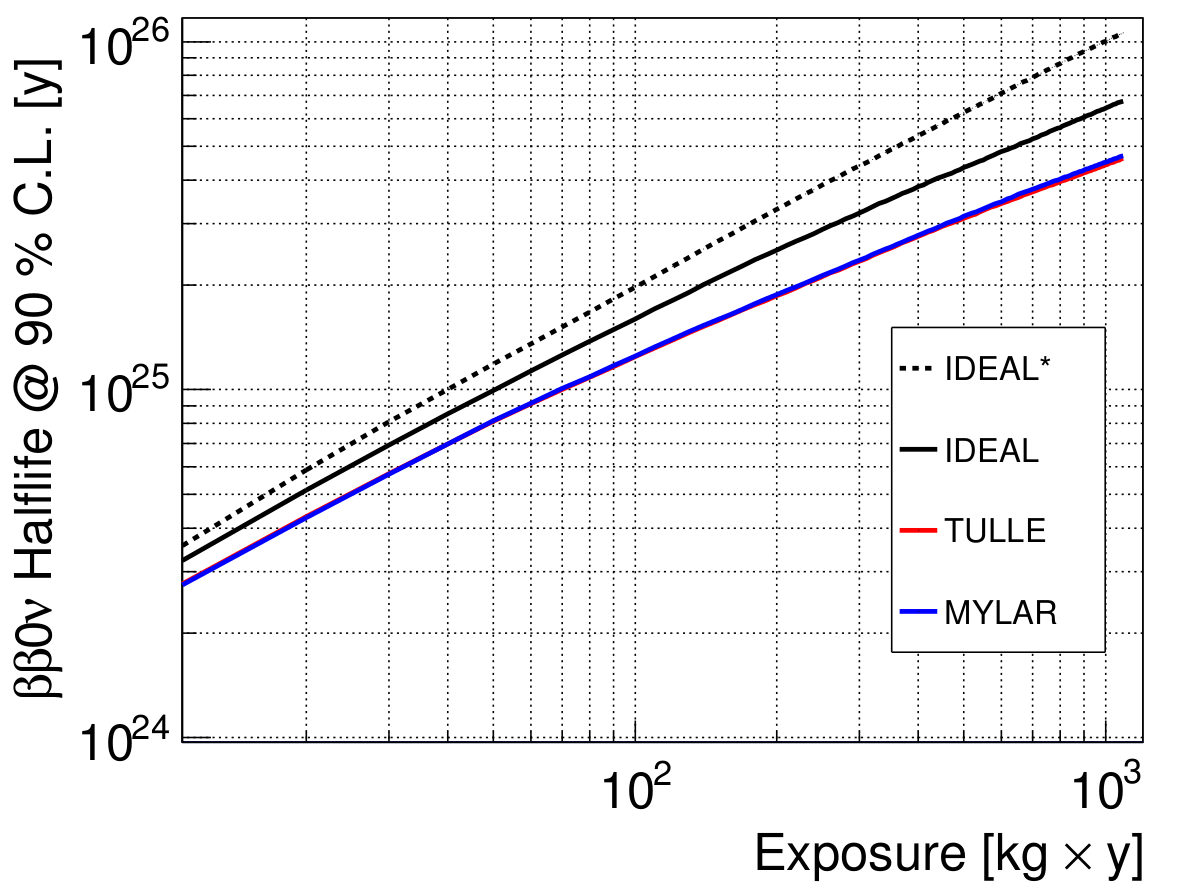
\includegraphics[scale=0.25]{pictures/Chap4/SensVsExposure3Designs.png}
\label{SensVsExposure3Designs.png}
\caption{SuperNEMO 0$\nu\beta\beta$ half-life limit at 90\% C.L. as a function of the exposure for the different designs of the source foil under consideration. The dotted line refers to the IDEAL design of the foil in which the backgrounds are normalised to the target radio-purity level of SuperNEMO.}
\end{figure}


\NI As discussed in sec. 3.3, the design of the source foil does not have a strong impact on the shape of the signal and background energy distributions. Nonetheless, the different activities of the material considered for the foil production and their mass fraction with respect to the 82 Se affect in a non negligible way the performance of SuperNEMO. With respect to the IDEAL design, the performance decreases by about 16\% for the TULLE design and about 16\% for the MYLAR design. The TULLE and the MYLAR design are compatible within 3\%. The plot in fig. 5.4 shows the extrapolation of the SuperNEMO sensitivity beyond the exposure expected for the demonstrator module, up to 1000 kg$\times$y.


\bigskip


\NI The comparison performed so far neglects the residual contamination of 208 Tl and 214 Bi expected in the 82 Se powder, since any value is available at present. Since no major improvement has been obtained, or proven, in the 82 Se purification process so far, the 82 Se contamination could be the dominant contribution to the background, regardless the design of the source foil. In tab. 5.2 the performance of SuperNEMO has been studied considering an additional contamination of 100 $\mu$Bq/kg both in 208 Tl and 214 Bi, as it could be expected from the 82 Se . The overall effect is a reduction of the discrepancies observed among the source foil design down to 11\% and 13\% for the TULLE and the MYLAR respectively. A high contamination of the 82 Se would then make the choice of the source foil design rather equivalent. This study will be updated as soon as the radio-purity measurement of the 82 Se powder will be available.


\begin{table}
\centering
\begin{tabular}{c|c|c|c|c}
\toprule
Design & R.O.I [keV] & $\epsilon_{\text{0}\nu}$ [\%] & bkg. [cts.] &   T$_{\text{1/2}}^{\text{0}\nu}$ [$\times$ 10$^{\text{24}}$~y] \\[0.1cm]
\hline
IDEAL           & [2700 ; 2980] & 19.47 $\pm$ 0.04 & 4.9 $\pm$ 0.2 & 3.8 \\  [0.1cm]
\hline
TULLE           & [2700 ; 3000] & 17.20 $\pm$ 0.04 & 6.3 $\pm$ 0.2 & 3.5 \\  [0.1cm]
\hline
MYLAR           & [2700 ; 3980] & 17.68 $\pm$ 0.04 & 6.0 $\pm$ 0.2 & 3.4 \\  [0.1cm]
\bottomrule
\end{tabular}
\caption{SuperNEMO demonstrator performance in 21 kg$\times$y considering an additional contamination of 100 $\mu$Bq/kg both in 208 Tl and 214 Bi to mimic the effect of an high contamination from 82 Se powder.}
\label{SNperformanceDiffDesign2}
\end{table}


\FloatBarrier


\subsection{Optimising the amount of PVA}


\NI In this section the optimal amount of PVA to mix with 82 Se during the production of the TULLE design is optimised in order to provide compatible performance with respect to the alternative MYLAR design. As shown in tab. 5.3, the variation of the amount of glue impact the thickness of the foil, i.e. the shape of the signal and background p.d.f. as shown in fig. 5.5, as well as the background level. The values in tab. 5.4 summarise the results of the performance study as a function of the amount of glue.


\bigskip


\NI Even if the best performances are obtained without glue, such scenario is not technically feasible since the 82 Se foil will not be resistant enough. A TULLE foil containing 5\% of PVA would still be compatible to the IDEAL design within 10\%, but it would be very hard to produce it, as observed during the R\&D tests at LAPP. From the technical point of view, a fraction of 10-15\% of PVA seems more reasonable and would allow to achieve performance compatible to the MYLAR design within 10\%.


\begin{table}
\centering
\begin{tabular}{c|c|c|c|c}
\toprule
f$_{\text{PVA}}$ & R.O.I [keV] & $\epsilon_{\text{0}\nu}$ [\%] & bkg. [cts.] &   T$_{\text{1/2}}^{\text{0}\nu}$ [$\times$ 10$^{\text{24}}$~y] \\[0.1cm]
\hline
0.00 & [2720 ; 3040] & 17.84 $\pm$ 0.04 & 0.9 $\pm$ 0.1 & 6.03 \\ [0.1cm]
\hline
0.05 & [2700 ; 3020] & 18.31 $\pm$ 0.04 & 2.0 $\pm$ 0.1 & 5.01 \\ [0.1cm]
\hline
0.10 & [2720 ; 3020] & 16.98 $\pm$ 0.04 & 2.3 $\pm$ 0.1 & 4.47 \\ [0.1cm]
\hline
0.15 & [2700 ; 2980] & 16.27 $\pm$ 0.04 & 3.3 $\pm$ 0.2 & 3.85 \\ [0.1cm]
\hline
0.20 & [2680 ; 3020] & 16.51 $\pm$ 0.04 & 5.7 $\pm$ 0.3 & 3.26 \\ [0.1cm]
\bottomrule
\end{tabular}
\caption{SuperNEMO performances with TULLE foils containing different amount of PVA.}
\label{Tab:AmountOfPVA}
\end{table}


\begin{figure}[h!]
\centering
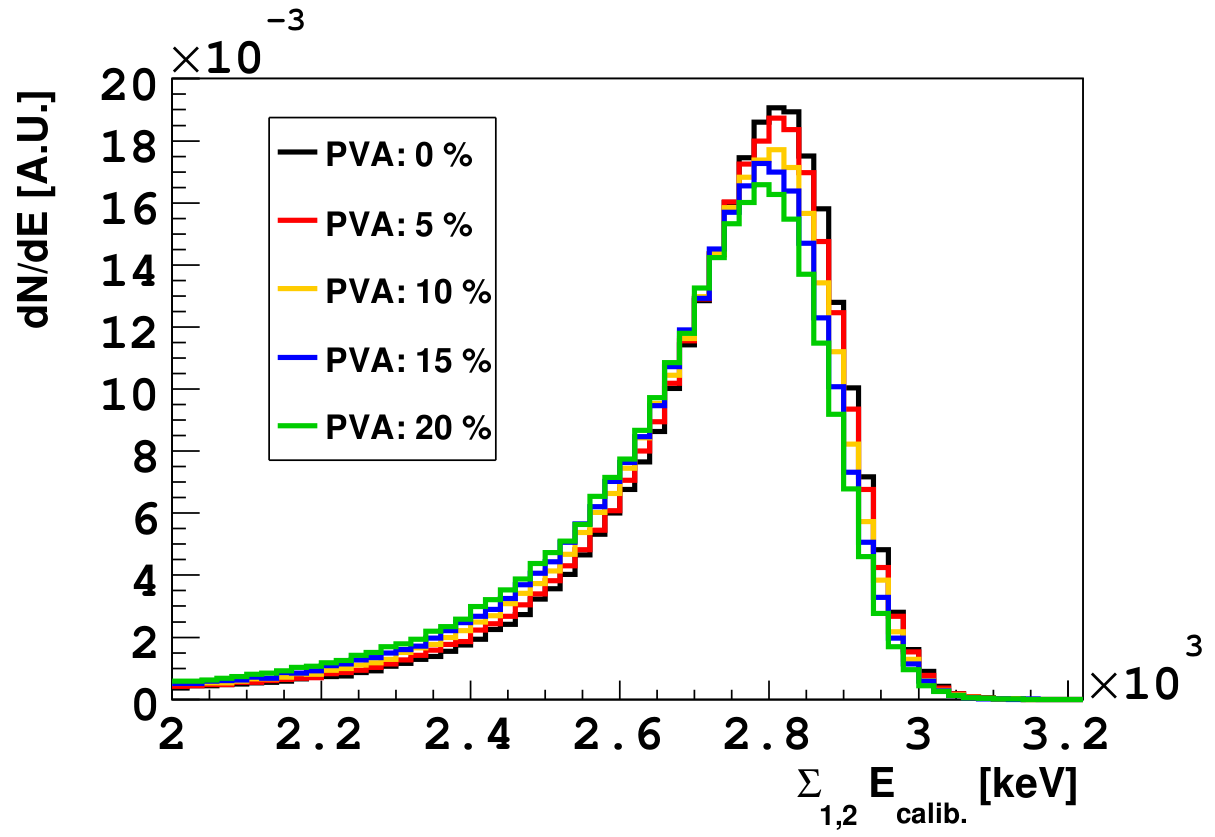
\includegraphics[scale=0.25]{pictures/Chap4/SpectrumPVA.png}
\label{SpectrumPVA.png}
\caption{0$\nu\beta\beta$ p.d.f. with TULLE foils containing different amount of PVA. The increased amount of PVA shifts the p.d.f. toward lower energies, due to an increased e energy loss in a thicker foil.}
\end{figure}


\subsection{Foil uniformity}


\NI The thickness of the source foil impact the energy losses of the out-coming particles worsening the resolution on the energy measurement. For similar reasons, the thickness impacts also the probability of observing 2e events from the beta decay of 208 Tl and 214 Bi . During the production of the source foil, the 82 Se + PVA paste is poured on a dedicated support and spread uniformly over the surface. Since the process is performed manually, a non uniform deposition of the paste may happen. This will cause a non uniform thickness over the foil length affecting the performance of the SuperNEMO demonstrator in terms of background level and sensitivity. For this reason is important to study such effects in order to define the acceptable level of uniformity of the source foil.


\subsubsection{Signal and background vs foil thickness}


\NI Signal and background events has been simulated considering a TULLE foil design containing 90\% of 82 Se and 10\% of PVA. The reference thickness of 190 $\mu$m has been varied by $\pm$10\% and $\pm$20\%. For each foil thickness, the simulated sample consists of 10 6 0$\nu\beta\beta$ events and 10 7 events for each background channel, 2$\nu\beta\beta$ , 208 Tl and 214 Bi . The expected energy spectra of the 2e  channel are shown in fig. 5.6 for the different thicknesses. It appear clearly looking at the 0$\nu\beta\beta$ (top left) and the 2$\nu\beta\beta$ top right) spectra of fig. 5.6 that the overall effect is a worsening of the energy resolution (increasing of the 0$\nu\beta\beta$ peak width) and a shift of the events toward lower energies due to a increase of the energy lost within the foil. Tab. 5.5 summarises the impact of the source foil thickness on the selection efficiency for the signal and the backgrounds. The selection efficiency being defined as the fraction of events satisfying the simple selection criteria of two reconstructed negative tracks hitting two calo blocks with a total energy deposition E $\beta\beta$ > 2 MeV. Uncertainties on the efficiencies are statistical only. Tab. 5.6 shows the same observables obtained for E $\beta\beta$ in 0$\nu$ . [2700; 3000] MeV, defined as the ROI maximising the sensitivity to T 1/2 The total background level and the best sensitivity obtained in the ROI are summarised in Tab. 5.7.


\begin{figure}[h!]
\centering
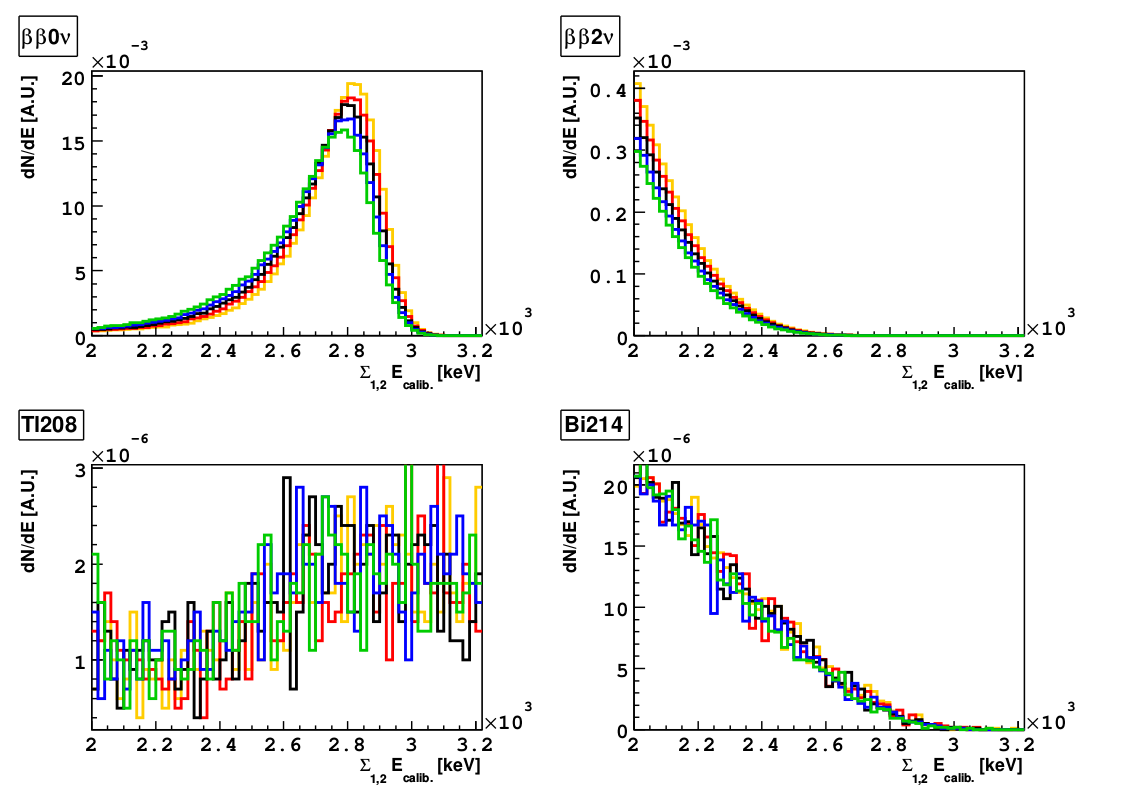
\includegraphics[scale=0.35]{pictures/Chap4/PVAspectra.png}
\label{PVAspectra.png}
\caption{Signal and background p.d.f. generated with different thickness of the source foil: 150 $\mu$m (yellow), 170 $\mu$m (red), 190 $\mu$m (black), 210 $\mu$m (blue), 220 $\mu$m (green)}
\end{figure}


\subsubsection{Effects of the foil uniformity}


\NI To mimic the effect of a non uniform foil thickness, we consider a case in which half of the foil is, for example, +10\% thicker and the other half is -10\% thinner than the nominal value. The average thickness of such a foil is still the nominal value and the amount of 82 Se + PVA paste required to produce it would be unchanged. The overall effect of such a non uniformity on a generic observable x is then obtained by averaging the same observable x + and x - obtained for the thicker and the thinner foil respectively. The relative comparison against the same observable obtained with the nominal thickness allows to obtain the systematic effect $\sigma$ due to the non uniformity:


\begin{equation}
\langle \text{x} \rangle = \text{x}_+ \left( \frac{\text{t}_+}{\text{t}_+ + \text{t}_-}  \right) + \text{x}_- \left( \frac{\text{t}_-}{\text{t}_+ + \text{t}_-}  \right) 
\end{equation}


\begin{equation}
\sigma_\text{x} = \frac{|\langle \text{x}\rangle - \text{x}|}{\text{x}}
\end{equation}


\bigskip


\NI The red and the blue histograms in fig. 5.7 show the averaged spectra obtained varying the foil thickness by $\pm$10\% and $\pm$20\% respectively. The black histogram shows the expected spectra at the nominal thickness of 190 $\mu$m. Tab. 5.8 shows the systematic effects on the signal and background selection efficiencies induced by a foil non uniformity for E $\beta\beta$ in [2000; 3100] keV. The effect of a variation of the foil thickness by $\pm$20\% is 0.5\% for the 0$\nu\beta\beta$ while it is slightly higher for the background events, remaining however within the statistical uncertainty of the simulated samples of about 5\%.


\begin{table}
\centering
\begin{tabular}{c|c|c}
\toprule
t [$\mu$m] & Bkg. [cts.] &  T$_{\text{1/2}}^{\text{0}\nu}$ [$\times$ 10$^{\text{24}}$~y] \\[0.1cm]
\hline
150 & 3.3 $\pm$ 0.2 & 4.63 \\[0.1cm]
170 & 3.0 $\pm$ 0.2 & 4.46 \\[0.1cm]
190 & 2.5 $\pm$ 0.1 & 4.41 \\[0.1cm]
210 & 2.4 $\pm$ 0.1 & 4.15 \\[0.1cm]
230 & 2.1 $\pm$ 0.1 & 4.01 \\[0.1cm]
\bottomrule
\end{tabular}
\caption{Background level and best sensitivity for E in [2700; 3000] keV.}
\label{Tab:ThicknessInfluence}
\end{table}


\bigskip


\NI Tab. 5.9 shows the effects in [2700; 3000] keV, where the best sensitivity is found. The effect of the thickness uniformity on the 0$\nu\beta\beta$ sample is < 3\% while for 2$\nu\beta\beta$ it increases up to 6\%. For the other internal background, the effect is < 8\%. The overall effect on the sensitivity is < 3\%. Assuming the systematic uncertainty on the signal and background efficiencies of 7\% and 10\% respectively [6] as the upper limit for the SuperNEMO demonstrator module, it is recommendable to aim for an uniformity <20\% over the whole foil surface. The effect of a $\pm$20\% uniformity remains in fact within the expected systematic uncertainties. In any case, it must be kept into account that the uniformity effects highlighted in this work could be reduced and perhaps neglected through a precise knowledge of the foil average thickness and a thickness map. Such a knowledge could be easily obtained through a dedicated measurement campaign (5\% at 200 $\mu$m) and then introduced in the geometry model of the SuperNEMO simulation software.


\begin{table}[h!]
\centering
\begin{tabular}{c|c|c|c|c|c}
\toprule
\multirow{2}{*}{Uniformity} & $\sigma_{\epsilon \text{0}\nu}$ & $\sigma_{\epsilon \text{2}\nu}$ & $\sigma_{\epsilon \text{Tl}}$ & $\sigma_{\epsilon \text{Bi}}$ & $\sigma_{\text{T1/2}}$ \\
  & [\%]  & [\%]  & [\%]  & [\%]  & [\%]  \\[0.1cm]
% [\%] & [\%] & [\%] & [\%] & [\%] & [\%] \\
\hline 
$\pm$10\% & 0.9 & 5.4 & 5.2 & 8.4 & 2.8 \\[0.1cm]
\hline 
$\pm$20\% & 2.8 & 6.0 & 3.4 & 4.2 & 3.3 \\[0.1cm]
\bottomrule
\end{tabular}
\caption{Systematic effect on signal and background efficiencies induced by non-uniformity of the source foil thickness for E  in [2700; 3000] keV.}
\label{Tab:SystematicInfluence}
\end{table}




\begin{figure}[h!]
\centering
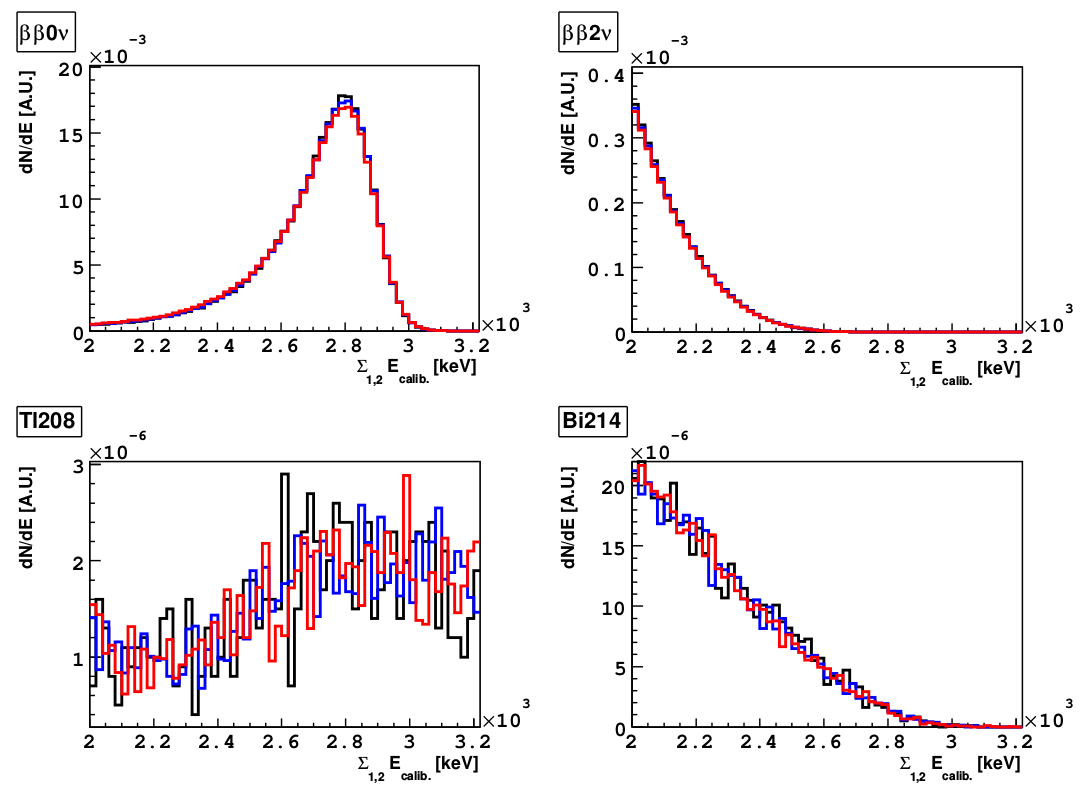
\includegraphics[scale=0.3]{pictures/Chap4/SpectrumThickness.png}
\label{SpectrumThickness.png}
\caption{The red and the blue histograms show the expected spectra obtained by averaging the spectra obtained variating the foil thickness by $\pm$10\% and $\pm$20\% respectively. The black histogram shows the expected
spectra at the nominal thickness of 190 $\mu$m.}
\end{figure}


\FloatBarrier


\section{Conclusion}\label{sec:SourceFoilDesignConclusion}


\NI The sensitivity of the SuperNEMO detector to the 0$\nu\beta\beta$ decay of 82 Se has been studied for different source foil designs. The different characteristics of the foils under consideration have been introduced with detail in chap. 2. The performance achievable with the TULLE and the MYLAR designs are compared to the IDEAL case in which the foil does not have any mechanical support. The event simulation and the recipe for the sensitivity calculation have been introduced in chap. 3 and chap. 4 respectively. The Falaise legacy software used in this work for the event simulation has not been fully validated here. A qualitative comparison with older studies shows however that the results are compatible. Anyway, the optimisation of the source foil design does not require an absolute validation of the simulation code as far as a relative comparison among the different designs is considered. Finally, in chap. 5 the performance of the SuperNEMO demonstrator module is studied. The design of the source foil does not have a strong impact on the shape of the energy distributions within the statistical uncertainties of the generated samples, 0.2\% and 5\% for signal and background respectively. Nonetheless, the different activities of 208 Tl and 214 Bi in the materials considered for the foil production and their mass fraction with respect to the 82 Se affect in a non negligible way the performance of SuperNEMO. With respect to the IDEAL design, the performance decreases by about 17\% and 22\% for the TULLE and the MYLAR design respectively. The TULLE and the MYLAR designs are compatible within 3\% among them. The differences among the designs decrease as the activities in 208 Tl and 214 Bi increase, making the choice of the source foil design rather equivalent in case of an high contamination coming, for example, from the 82 Se . The effect of a non uniformity on the thickness of the source foil has also been studied. The result of the sensitivity calculation performed for different thicknesses of the foil recommends an uniformity <20\% over the whole foil surface.



















\end{document}
